\section{ Balistic flight over earth:Non rotating Spherical.elips.polar.law of conserv }\label{sec:q3}    
\begin{enumerate}[label=(\alph*)]
\item
$\gamma_0$ - Initial flight path angle\\
$V_0$ - Velocity at launch\\
$\theta_0$ - Initial true anomaly\\
$R_e$ - Radius of earth\\
$a$ - semi-major axis\\
$r_a$ - apogee height\\
$r_p$ - Perigee height\\
AE - Flight range

The figure can be found in Lecture 8, Slide 35.\\
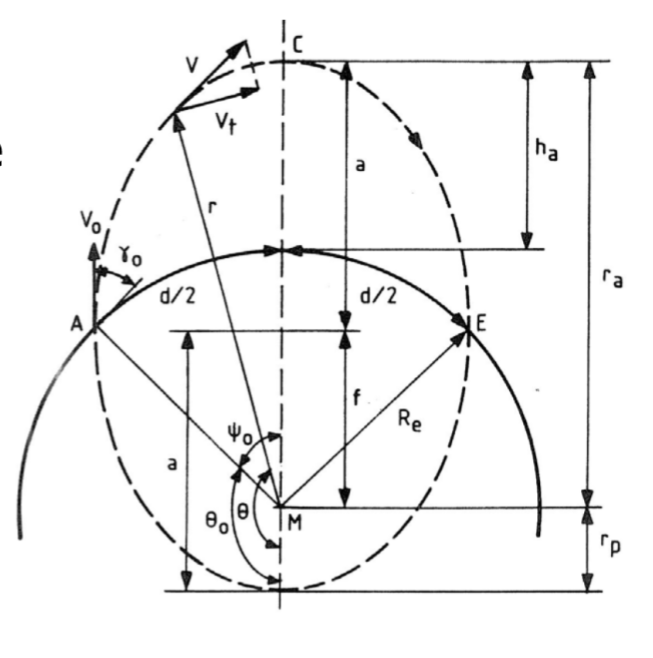
\includegraphics[scale=0.6]{3a.PNG}

\item
At launch conditions, orbital momentum per unit mass, H can be written as $H=R_eV_0cos\gamma_0$. the equation of conservation of orbital energy yields,
$$\frac{V_0^2}{2}-\frac{\mu}{R_e}=-\frac{\mu}{2a}$$
$$\Rightarrow \frac{R_e}{a}=2-\frac{V_0^2R_e}{\mu}$$
But we know that the dimensionless launch velocity $S_0=\frac{V_0}{\sqrt{\mu/R_e}}=0.695$. Therefore, $$\frac{a}{R_e} = \frac{1}{2-S_0^2}$$
It is also known that $p=H^2/\mu$. Therefore,
$$\frac{p}{R_e}=\frac{H^2}{\mu R_e}=S_0^2 cos^2 \gamma_0$$
Eccentricity, $e=\sqrt{1-p/a}=\sqrt{1-S_0^2cos^2 \gamma_0(2-S_0^2)}$.
The apogee altitude, $h_a$ can be derived as
$$h_a = r_a-R_e = a(1+e)-R_e = \frac{R_e}{2-S_0^2}(1+\sqrt{1-S_0^2cos^2\gamma_0(2-S_0^2)})-R_e$$
$$\Rightarrow \frac{h_a}{R_e} = \frac{S_0^2+\sqrt{1-S_0^2cos^2\gamma_0(2-S_0^2)}-1}{2-S_0^2}=0.2335$$
Apogee altitude, $h_a=1487.316\: km$

\item
At any point in the trajectory, the position of the rocket can be given by, $r=\frac{p}{1+ecos\theta}$
At launch point, $$R_e = \frac{R_eS_0^2cos^2\gamma_0}{1+cos\theta_0\sqrt{1-S_0^2cos^2\gamma_0(2-S_0^2)}}$$
$$\Rightarrow 1 = \frac{S_0^2cos^2\gamma_0}{1+cos\theta_0\sqrt{1-S_0^2cos^2\gamma_0(2-S_0^2)}}$$
$$\Rightarrow cos\theta_0 = \frac{S_0^2cos^2\gamma_0-1}{\sqrt{1-S_0^2cos^2\gamma_0(2-S_0^2)}}$$
If $d/2$ is the semi-shooting range, then 
$$\pi-\theta_0 = \frac{d/2}{R_e}$$
$$\Rightarrow d=2R_e(\pi-\theta_0) = 2R_ecos^{-1}\frac{S_0^2cos^2\gamma_0-1}{\sqrt{1-S_0^2cos^2\gamma_0(2-S_0^2)}}=36666.273\: km$$
 
\item
$\lambda$ - Latitude\\
$\Lambda$ - Longitude\\
$\beta_0$ - Launch angle (Azimuth)\\
$i$ - Inclination angle\\
$\hat{d}$ - Dimensionless shooting range\\
$\Omega$ - Longitude of ascending node\\
$\hat{d}$ - Dimensionless shooting range\\
This figure is taken from Lecture 9, Slide 10.\\
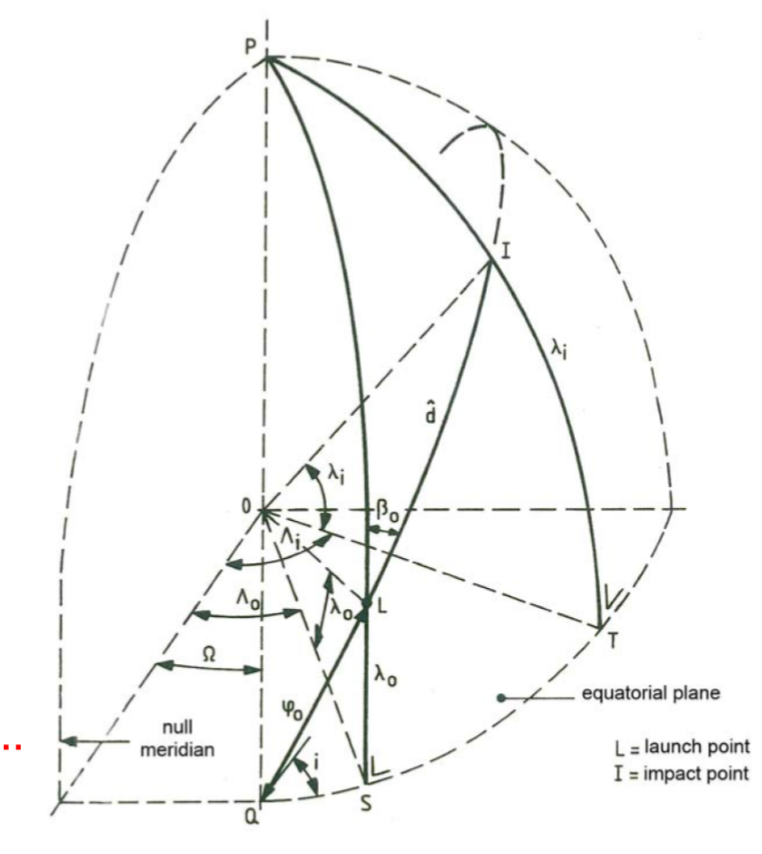
\includegraphics[scale=0.6]{3d}

\item
\textbf{Expression for inclination of orbit}\\

Applying Napier rule (R8) on $\triangle QLS$
$$\cos i = \sin\beta_0 \cos\lambda_0=0.5332$$
$$\Rightarrow i=57.78^\circ $$

\textbf{Relationship between RAAN ($\Omega$) and initial launch parameters}\\

Applying Napier rule (R7) on $\triangle QLS$
$$\tan \lambda_0 = \cos\beta_0 \tan\phi_0$$
$$\Rightarrow \tan \phi_0 = \frac{\tan\lambda_0}{\cos\beta_0}=-2.5599$$
$$\Rightarrow \phi_0=-68.6623^\circ$$
Using Napier rule R6,
$$\tan(\Lambda_0-\Omega)=\cos i \tan\phi_0 = \sin\beta_0 \cos\lambda_0\frac{\tan\lambda_0}{\cos\beta_0}$$
$$\Rightarrow \tan(\Lambda_0-\Omega)=\sin\lambda_0 \tan\beta_0=-1.3649$$
$$\Rightarrow \Omega=\Lambda_0-\arctan(-1.3649)=58.7710^\circ E$$
\item
\textbf{Latitude at point of impact}
Applying cos rule to  $\triangle LPI$
$$\cos(\pi/2-\lambda_i)=\cos(\pi/2-\lambda_0)\cos\hat{d}+\sin(\pi/2-\lambda_0)\sin\hat{d}\cos\beta_0$$
$$\Rightarrow \sin\lambda_i = \sin\lambda_0\cos\hat{d}+\cos\lambda_0\sin\hat{d}\cos\beta_0=0.8359$$
$$\lambda_i=56.7098^\circ N$$

\textbf{Longitude at point of impact}
Applying Napier rule R6 on $\triangle QIT$
$$\tan(\Lambda_i-\Omega)=\cos i \tan(\phi_0+\hat{d})=3.4195$$
$$\Rightarrow \Lambda_i = 132.4698^\circ E$$
where the expression for $\hat{d}=\frac{d}{Re}$ is same as in question 3c.
\end{enumerate}